% !TEX encoding = UTF-8
% !TEX TS-program = pdflatex
% !TEX root = ../../tesi.tex

\section{Prodotti}
Per quanto concerne i prodotti, ho discusso con il mio \textit{tutor} aziendale, Fabio Pallaro, il quale mi ha specificato che tutti i prodotti sono stati sviluppati per aiutare le aziende ad affrontare i cambiamenti tecnologici e di mercato, rimanendo sempre competitive nell'attuale contesto di trasformazione digitale. I settori informatici dove opera principalmente l'azienda sono: il \textit{business consultancy}, il \textit{IT consultancy} e il \textit{project financing}.

\begin{figure}[!h]
  \centering
  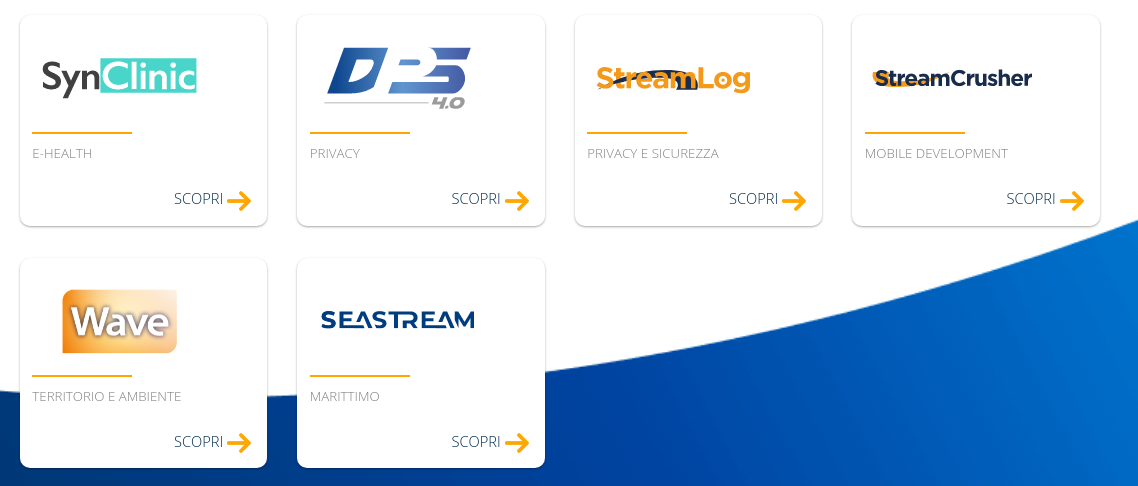
\includegraphics[width=\textwidth]{capitolo1/prodotti-synclab.png}
  \caption{I prodotti di Sync Lab}
  \textbf{Fonte}: \href{https://www.synclab.it/prodotti.php}{https://www.synclab.it/prodotti.php}
\end{figure}

\noindent In questo ambito, Sync Lab, ha sviluppato numerosi prodotti:
\begin{itemize}
  \item \textbf{SynClinic}: \textit{software} che facilita la gestione di una struttura sanitaria. Utilizzabile in \textit{cloud} e \gls{on premises}, gestisce, organizza e monitora tutte le fasi del percorso di cura del paziente, integrandosi perfettamente con i servizi regionali: fascicolo sanitario elettronico, ricetta dematerializzata e CUP regionale;
  
  \item \textbf{DPS 4.0}: consiste in una soluzione web per la gestione del GDPR, con una piattaforma guidata per aggiornare e modificare automaticamente i documenti di privacy in modo conforme agli standard di riferimento europei;
  
  \item \textbf{StreamLog}: rappresenta un sistema finalizzato al soddisfacimento dei requisiti fissati al garante, ovvero effettua il controllo degli accessi ai sistemi in modo semplice e veloce. La piattaforma è basata su \textit{framework open source} allo stato dell'arte e, in particolare, su un'innovativa tecnologia di \textit{streaming}, frutto del laboratorio di ricerca e sviluppo Sync Lab;
  
  \item \textbf{StreamCrusher}: soluzione \textit{software} che è in grado di raccogliere, indicizzare, ed interpretare la grande mole di dati che giornalmente genera qualsiasi azienda. In seguito, produrrà un resoconto con tutte le informazioni utili al centro informatico, per identificare criticità o eventuali opportunità di \textit{business};
  
  \item \textbf{Wave}: nato dal laboratorio di ricerca e sviluppo, è un \textit{plugin} della piattaforma \textit{Milestone System A/S} che permette di avere una visione geografica della distribuzione delle telecamere installate nel territorio e di capire la copertura garantita da un'installazione reale;
  
  \item \textbf{SeaStream}: piattaforma che migliora l'efficienza, la sicurezza e il processo di innovazione del settore marittimo, mettendo a disposizione strumenti per il monitoraggio e tracciamento delle navi e per la gestione portuale.  
\end{itemize}